\documentclass{article}

\usepackage{graphicx}          % Para graficos
\usepackage{hyperref}          % Para meter hipervinculos
\usepackage{soul}

\graphicspath{ {./informe/images/} }

\begin{document}

\begin{titlepage}
  \vspace*{1cm}

  \begin{center}
    {\Huge{Trabajo Práctico 2: Software-Defined Networks}}
  \end{center}

  \vspace{0.4cm}

  \begin{center}
    {\LARGE{Facultad de Ingeniería de la Universidad de Buenos Aires}}\\
    \vspace{0.3cm}
    {\Large{Redes}}\\
    \vspace{0.3cm}
    {\large{Cátedra Hamelin-Lopez Pecora}}\\
  \end{center}

  \vspace{0.8cm}
  \begin{center}
    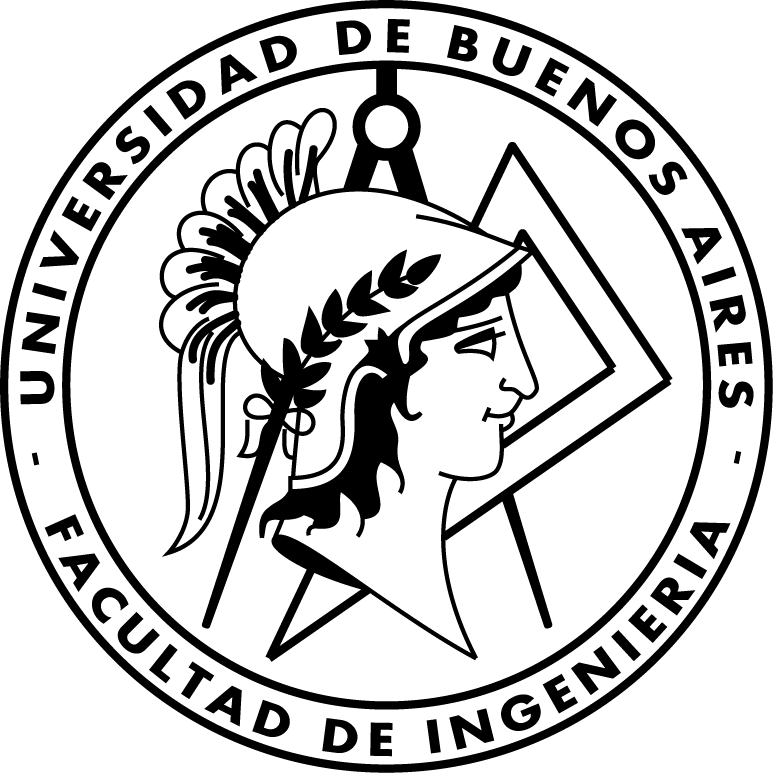
\includegraphics[scale=0.8]{Logo-fiuba}
  \end{center}

  \vspace{1.4cm}
  \begin{center}

    {\begin{minipage}{.5\textwidth}
        \begin{center}
          Demarchi, Ignacio\\
          {\small{Padrón: 107835}}\\
          {\small{email: idemarchi@fi.uba.ar}}\\
        \end{center}
      \end{minipage}\begin{minipage}{.5\textwidth}
        \begin{center}
          Lijs, Theo\\
          {\small{Padrón: 109472}}\\
          {\small{email: tlijs@fi.uba.ar}}
        \end{center}
      \end{minipage}}

    \vspace{1.0cm}

    {\begin{minipage}{.5\textwidth}
        \begin{center}
          Schneider, Valentin\\
          {\small{Padrón: 107964}}\\
          {\small{email: vschneider@fi.uba.ar}}\\
        \end{center}
      \end{minipage}\begin{minipage}{.5\textwidth}
        \begin{center}
          Orsi, Tomas Fabrizio\\
          {\small{Padrón: 109735}}\\
          {\small{email: torsi@fi.uba.ar}}
        \end{center}
      \end{minipage}}

  \end{center}
\end{titlepage}

% \renewcommand*\contentsname{Indice}
\tableofcontents
\pagebreak

\section{\texorpdfstring{\textbf{Introducción}}{Introducción}}\label{introducciuxf3n}


\section{\texorpdfstring{\textbf{Hipótesis y suposiciones realizadas}}{Hipótesis y suposiciones realizadas}}\label{hipuxf3tesis-y-suposiciones-realizadas-wip}


\section{\texorpdfstring{\textbf{Herramientas utilizadas}}{Herramientas utilizadas}}\label{implementaciuxf3n-wip}

\subsection{Mininet}\label{arquitectura-cliente-servidor}

aca describir la topologia, como se arma todo (pero el comando en el readme nomas)

\subsection{POX}\label{socketrdt}
explicar como es que levanta y aplica las reglas, el formato de las reglas
y como conecta a lo que este corriendo en mininet

\subsection{Wireshark \& iperf}\label{stop-and-wait}
explicar por encima que al tener mininet abierto
desde wireshark podemos elegir esa red (o lo que sea que es)
y ver los paquetes ya que se mandan con los protocolos de siempre,
si usamos el ping de mininet vemos ICMP, y si usamos iperf
vamos a ver TCP/UDP.
a iperf lo corremos dentro de los hosts de mininet

\section{\texorpdfstring{\textbf{Resultados de simulaciones}}{Resultados de simulaciones}}\label{pruebas-wip}

\subsection{Puerto Destino 80}
Simulacion para descartar todos los mensajes cuyo puerto destino sea 80.

\subsubsection{Reglas}
\begin{center}
\includegraphics[scale=0.35]{UploadJoseph.jpg(6,5MB)conStopWait}
\end{center}

\subsubsection{Wireshark}
\begin{center}
\includegraphics[scale=0.35]{UploadJoseph.jpg(6,5MB)conSelectiveRepeat}
\end{center}

\subsubsection{Logs del controlador}
\begin{center}
\includegraphics[scale=0.35]{DownloadGrupo12.png(1,2MB)conStopWait}
\end{center}


\subsection{Host 1, Puerto 5001 y UDP}
Simulacion para descartar todos los mensajes que provengan del host 1, tengan como puerto destino el 5001, y esten utilizando el protocolo UDP.

\subsubsection{Reglas}
\begin{center}
\includegraphics[scale=0.35]{UploadJoseph.jpg(6,5MB)conStopWait}
\end{center}

\subsubsection{Wireshark}
\begin{center}
\includegraphics[scale=0.35]{UploadJoseph.jpg(6,5MB)conSelectiveRepeat}
\end{center}

\subsubsection{Logs del controlador}
\begin{center}
\includegraphics[scale=0.35]{DownloadGrupo12.png(1,2MB)conStopWait}
\end{center}

\subsection{Dos hosts no se comunican entre si}
Simulacion donde se eligen dos hosts cualquiera, y los mismos no pueden comunicarse de ninguna forma.

\subsubsection{Reglas}
\begin{center}
\includegraphics[scale=0.35]{UploadJoseph.jpg(6,5MB)conStopWait}
\end{center}

\subsubsection{Wireshark}
\begin{center}
\includegraphics[scale=0.35]{UploadJoseph.jpg(6,5MB)conSelectiveRepeat}
\end{center}

\subsubsection{Logs del controlador}
\begin{center}
\includegraphics[scale=0.35]{DownloadGrupo12.png(1,2MB)conStopWait}
\end{center}


\section{\texorpdfstring{\textbf{Preguntas a responder}}{Preguntas a responder}}\label{preguntas-a-responder}

\subsection{\texorpdfstring{\textbf{¿Cuál es la diferencia entre un Switch y un router? ¿Qué tienen en común?}}{1. ¿Cuál es la diferencia entre un Switch y un router? ¿Qué tienen en común?}}\label{describa-la-arquitectura-cliente-servidor.}


\subsection{\texorpdfstring{\textbf{¿Cuál es la diferencia entre un Switch convencional y un Switch OpenFlow?}}{¿Cuál es la diferencia entre un Switch convencional y un Switch OpenFlow?}}\label{detalle-el-protocolo-de-aplicaciuxf3n-desarrollado-en-este-trabajo.}


\subsection{\texorpdfstring{\textbf{¿Se pueden reemplazar todos los routers de la Intenet por Switches OpenFlow? Piense en el escenario interASes para elaborar su respuesta}}{¿Se pueden reemplazar todos los routers de la Intenet por Switches OpenFlow? Piense en el escenario interASes para elaborar su respuesta}}\label{la-capa-de-transporte-del-stack-tcpip-ofrece-dos-protocolos-tcp-y-udp.-quuxe9-servicios-proveen-dichos-protocolos-cuuxe1les-son-sus-caracteruxedsticas-cuuxe1ndo-es-apropiado-utilizar-cada-uno}


\section{\texorpdfstring{\textbf{Dificultades
encontradas}}{Dificultades encontradas}}\label{dificultades-encontradas}

\section{\texorpdfstring{\textbf{Conclusión}}{Conclusión}}\label{conclusiuxf3n-wip}

\end{document}